\documentclass[11pt,paper=a4,answers]{exam}
\usepackage{
    graphicx, % For figures
    lastpage,
    upgreek,
    censor,
    amsmath,
    gensymb, % For symbols
    array, % For table types
    caption, % Allowing empty caption
    enumerate, % for indexing of alphabets/ romans
    cleveref
    }
\censorruledepth=-.2ex
\censorruleheight=.1ex
\hyphenpenalty 10000
\usepackage[paperheight=10.5in,paperwidth=8.27in,bindingoffset=0in,left=0.8in,right=1in,
top=0.7in,bottom=1in,headsep=.5\baselineskip]{geometry}
\flushbottom
\usepackage[normalem]{ulem}
\renewcommand\ULthickness{2pt}   %%---> For changing thickness of underline
\setlength\ULdepth{1.5ex}%\maxdimen ---> For changing depth of underline
\renewcommand{\baselinestretch}{1}
\pagestyle{empty}

\newcolumntype{M}[1]{>{\centering\arraybackslash}m{#1}}
\usepackage[most]{tcolorbox}

\pagestyle{headandfoot}

\headrule
\newcommand{\continuedmessage}{
    \ifcontinuation{\footnotesize Question \ContinuedQuestion\ continues\ldots}{}%
}
\runningheader{\footnotesize Mathematics}
{\footnotesize HKDSE 2024 --- Math Core Paper 1}
{\footnotesize Page \thepage\ of \numpages}

\footrule
\footer{\footnotesize Student's name:}

{\ifincomplete
    {\footnotesize Question \IncompleteQuestion\ continues on the next page\ldots}
    {\iflastpage{\footnotesize End of exam}{\footnotesize Please go on to the next page\ldots}}
}
\crefname{figure}{figure}{figures}
\crefname{question}{question}{questions}
%==============================================================
\begin{document}

\noindent
\begin{minipage}[r]{\textwidth}%
\begin{center}
    {\bfseries HONG KONG EXAMINATION \& ASSESSMENT AUTHORITY 
        \par \vspace{0.5cm}
        Hong Kong Diploma of Secondary Education Examination 2024
        \par
    \Large Mathematics (Compulsory Part) Paper 1 \\[2pt]
    \vspace{0.5cm}
    }
\end{center}
\end{minipage}
\par
\noindent
\uline{Time: 2 hours, 15 minutes   
\hfill Maximum Marks: 105}

\begin{center}
\fbox{\fbox{\parbox{5.5in}{\centering
            \textbf{2024 HKDSE Math Paper, 15 Apr 2024}
            \begin{itemize}
                \item Documented on \LaTeX, 16 Apr 2024 
                \item Good luck!
            \end{itemize}}}}
\vspace{0.1in}
\end{center}

\section*{Section A(1) ~~ (35 marks)}
\begin{questions}
    \pointsdroppedatright
    \marksnotpoints
    \bracketedpoints
    \marginpointname{ \points}

\vspace{0.5cm}
\label{2024-I-1: Fractions}
\question[3]
    Simplify $\displaystyle \frac{2}{4h-7} - \frac{3}{6h-5}$.
    \droppoints

\vspace{0.5cm}
\label{2024-I-2: Changing Subject}
\question[3] 
    Make $\displaystyle x$ the subject of the formula $\displaystyle \frac{Ax + C}{B} = 3x$.
    \droppoints

\vspace{0.5cm}
\label{2024-I-3: Factorization}
\question[3]
    Factorize
    \begin{parts}
        \vspace{0.2cm}
        \part 
            $\displaystyle 6r^2 - 13rs - 28s^2$,
        \vspace{0.2cm}
        \part 
            $\displaystyle 4r - 14s + 6r^2 - 13rs - 28s^2$.
    \end{parts}
    \droppoints

\vspace{0.5cm}
\label{2024-I-4: Inequalities}
\question[4]
    \begin{parts}
        \part 
            Find the range of values of $\displaystyle x$ which satisfy both
            $\displaystyle \frac{5x + 7}{4} - 1 < 2x$
            \text{and}
            $\displaystyle 3x + 9 \geq 0$.
        \vspace{0.2cm}
        \part 
            Write down the least integer satisfying both inequalities in (a).
    \end{parts}  
    \droppoints

\vspace{0.5cm}
\label{2024-I-5: Ratios}
\question[4]
    Let $\displaystyle a, b$ and  $\displaystyle c$ be non-zero numbers such that 
    $\displaystyle 5a = 6c$
    \text{and}
    $\displaystyle \frac{2b + 7c}{b + c} = 4$.
    Find 
    $\displaystyle \frac{5a + 8b}{2b + 3c}$
    \droppoints

\vspace{0.5cm}
\label{2024-I-6: Percentages}
\question[4]
    The marked price of a calculator is 40\% higher than its cost. The calculator is sold at a discount of 25\% on its marked price and the profit is $\$13$. 
    Find the marked price of the calculator.
    \droppoints

\newpage
\vspace{0.5cm}
\label{2024-I-7: Polar}
\question[4]
    In a polar coordinate system, $
    \displaystyle O$ is the pole. The polar coordinates of the points $\displaystyle P, Q$ and $\displaystyle R$ are
    $\displaystyle(11, 59\degree)$, $\displaystyle (60, 149\degree)$ and $\displaystyle (144, 239\degree)$ respectively.

    \begin{parts}
        \vspace{0.2cm}
        \part 
            Find $\displaystyle \angle POQ$.
        \vspace{0.2cm}
        \part 
            Are $\displaystyle P, O$ and $\displaystyle R$ collinear? Explain your answer.
        \vspace{0.2cm}
        \part
            Find the perimeter of $\displaystyle \Delta PQR$.
    \end{parts}  
    \droppoints

\vspace{0.5cm}
\label{2024-I-8: Congruence & Pyth}
\question[5]
    In Figure 1, $ \displaystyle E$ is the point of intersection of $\displaystyle AC$ and $\displaystyle BD$. 

    \begin{figure}[ht]
        \centering
        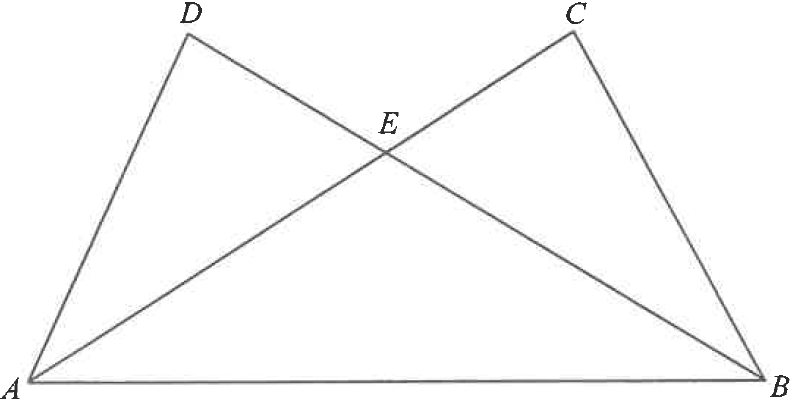
\includegraphics[width=0.5\linewidth]{figure_1.png}
        \caption*{Figure 1}
    \end{figure}

    It is given that 
    $\displaystyle \angle ACB = \angle ADB = 90\degree$ and $\displaystyle AD = BC$.
    
    \begin{parts}
        \vspace{0.2cm}
        \part 
            Prove that $\displaystyle \Delta ABC \cong \Delta BAD$.
        \vspace{0.2cm}
        \part 
            If $\displaystyle AD = 12$ cm and $\displaystyle DE = 9$ cm, find the area of the pentagon $\displaystyle ABCED$.
    \end{parts}  
    \droppoints

\vspace{0.5cm}
\label{2024-I-9: Stats/ Central Tendency}
\question[5]
    The table shows the distribution of the numbers of keys owned by a group of housewives.

    \begin{center}
        \begin{tabular}{|M{4cm}||M{1cm}|M{1cm}|M{1cm}|M{1cm}|M{1cm}|M{1cm}|}
        \hline
        Number of keys & 3 & 4 & 5 & 6 & 7 & 8 \\ \hline
        Number of housewives & 10 & 9 & 4 & 3 & 4 & $k$
        \\
        \hline
        \end{tabular}
    \end{center}

    If a housewife is randomly selected from the group, then the probability that she owns more than 6 keys is $\displaystyle \frac{5}{18}$.
    
    \begin{parts}
        \vspace{0.2cm}
        \part 
            Find $k$.
        \vspace{0.2cm}
        \part 
            Write down the mean, mode and median of the distribution.
    \end{parts}  
    \droppoints
\end{questions}

\newpage
\section*{Section A(2) ~~ (35 marks)}
    \marksnotpoints
\begin{questions}
    \setcounter{question}{9}
\label{2024-I-10: Variation}
\question
    It is given that $\displaystyle g(x)$ is partly constant and partly varies as $\displaystyle x$.

    Suppose that $\displaystyle g(-3) = -21$ and $\displaystyle g(7) = 9$.

    \begin{parts}
        \vspace{0.2cm}
        \part[3]
            Find $\displaystyle g(x)$. \droppoints
        \vspace{0.2cm}
        \part[3]
            Let $\displaystyle h(x) = xg(x) + k$, where $\displaystyle k$ is a real constant. 
            
            If all the roots of the equation $\displaystyle h(x) = 0$ are real numbers, find the range of values of $k$.
            \droppoints
    \end{parts}  

\vspace{0.5cm}
\label{2024-I-11: Stats/ Stem-leaf}
\question
    The stem-and-leaf diagram below shows the distribution of the numbers of hours spent on reading journals in a month by a group of researchers.

    \begin{center}
        \begin{tabular}{r|l}
        \underline{Stem (tens)} & \underline{Leaf (units)}
        \\       
        2 & 0 \quad 0 \quad 1 \quad $a$ \quad $a$ \quad $a$ \quad 8 \quad 8 \quad 9 \quad 9
        \\
        3 & 0 \quad 0 \quad 2 \quad 3 \quad 4 \quad 4 \quad 7 \quad 9
        \\
        4 & 0 \quad $b$
        \end{tabular}
    \end{center}

    \begin{parts}
        \part[3]
            Find $a$ and $b$. \droppoints
        \vspace{0.2cm}
        \part[1]
            Write down the least possible range of the distribution. \droppoints
        \vspace{0.2cm}
        \part[2]
            Find the greatest possible inter-quartile range of the distribution. \droppoints
    \end{parts}  

\vspace{0.5cm}
\label{2024-I-12: Locus}
\question
    Denote the origin by $O$.
    \begin{parts}
        \part[3]
            $A$ and $B$ are points lying on the positive $x$-axis such that the $x$-coordinate of $A$ is greater than the $x$-coordinate of $B$. A vertical line which passes through $B$ cuts the straight line $y = mx$ at the point $C$ such that $AB = BC$, where $m$ is a positive constant.

            \vspace{0.2cm}
            Let $D$ be a point such that $ABCD$ is a square. Express the slope of $OD$ in terms of $m$. \droppoints
        \part[4]
            The coordinates of the points $M$ and $N$ are (6, 5) and (10, 0) respectively. Let $P$ and $Q$ be points lying on $OM$ and $MN$ respectively while $R$ and $S$ be points lyings on the $x$-axis.

            \vspace{0.2cm}
            If the quadrilateral $PQRS$ is a square, find the $x$-coordinate of $P$. \droppoints
    \end{parts}

\newpage
\vspace{0.5cm}
\label{2024-I-13: Mensuration}
\question
    The base of a solid right pyramid is a square of side 64 cm. The height of a pyramid is 24 cm. The pyramid is divided into a frustum $X$ and a pyramid $Y$ by a plane parallel to its base.

    It is given that the height of $Y$ is 18 cm.
    \begin{parts}
        \part[3]
            Find the volume of $X$. \droppoints
        \part[4]
            The base of another solid right pyramid is a square. The pyramid is divided into a frustum $Z$ and a pyramid by a plane parallel to its base. The height and the total surface area of $Z$ are 3 cm and 960 cm$^2$ respectively.

            \vspace{0.2cm}
            Are $X$ and $Z$ similar? Explain your answer. \droppoints
    \end{parts}

\vspace{0.5cm}
\label{2024-I-14: Remainder Theorem}
\question
    Let $\displaystyle F(x) = (6x^2 + x + p)(qx^2 + rx - 10)$, where $p, q$ and $r$ are constants.

    The constant term of $F(x)$ is 40.
    \begin{parts}
        \part[1]
            \vspace{0.2cm}
            Write down the value of $p$. \droppoints
        \vspace{0.2cm}
        \part[7]
            When $F(x)$ is divided by $x + 1$, the remainder is $-12$. Given that $x - 2$ is a factor of $F(x)$.
            \begin{enumerate}[(i)]
                \vspace{0.2cm}
                \item 
                    Find $q$ and $r$.
                \item 
                    How many irrational roots does the equation $F(x) = 0$ have? Explain your answer.
            \end{enumerate} \droppoints
    \end{parts}    
\end{questions}

\newpage
\section*{Section B ~~ (35 marks)}
    \marksnotpoints
\begin{questions}
    \setcounter{question}{14}

    \label{2024-I-15: Log graph}
    \question[3]
        It is given that $\displaystyle \log_{9}y$ is a linear function of $\displaystyle \log_{3}x$. Denote the graph of the linear function by $L$.
        The slope of $L$ is 4 and $L$ passes through the point (5, 22).
        
        \vspace{0.2cm}
        Express $y$ in terms of $x$. \droppoints

    \vspace{0.5cm}
    \label{2024-I-16: Permutation and combination}
    \question
        In a bag, there are 16 red cups and 4 white cups. If 5 cups are randomly drawn from the bag at the same time, find
        \begin{parts}
        \part[2]
            \vspace{0.2cm}
            the probability that exactly 1 white cup is drawn, \droppoints
        \part[2]
            \vspace{0.2cm}
            the probability that at most 3 red cups are drawn. \droppoints
        \end{parts}

    \vspace{0.5cm}
    \label{2024-I-17: Locus and circle}
    \question
        The coordinates of the points $Q$ and $R$ are ($10, -1$) and ($-4, -9$) respectively.
        \begin{parts}
            \part[3]
                \vspace{0.2cm}
                Let $P$ be a moving point in the rectangular coordinate plane such that $PQ = PR$. 
                
                Denote the locus of $P$ by $\Gamma$.
                \begin{enumerate}[(i)]
                \vspace{0.2cm}
                \item 
                    Describe the geometric relationship between $\Gamma$ and $QR$.
                \vspace{0.2cm}
                \item 
                    Find the equation of $\Gamma$.
            \end{enumerate} \droppoints

            \vspace{0.2cm}
            \part[5]
                Let $C$ be the circle which passes through $Q$, $R$ and the point ($4, 3$).
                \begin{enumerate}[(i)]
                \vspace{0.2cm}
                \item 
                    Find the equation of $C$.
                \vspace{0.2cm}
                \item 
                    The coordinates of the point $U$ is (10, 4). It is found that $U$ lies outside $C$. $UV$ and $UW$ are the tangents to $C$ at the points $V$ and $W$ respectively.

                    \vspace{0.2cm}
                    Is the area of the circumcircle of $\Delta UVW$ greater than 100? Explain your answer.
            \end{enumerate} \droppoints   
        \end{parts}

    \newpage
    \label{2024-I-18: 3D Trigo}
    \question
        \begin{parts}
            \part[4]
                $PQRS$ is a thin quadrilateral metal sheet where $PQ = 12$cm, $PS = 10$cm, $QR = 13$cm, $\angle QPS = 82\degree$ and $\angle QRS = 65\degree$. Find
                \begin{enumerate}[(i)]
                    \item the length of $QS$,
                    \item $\angle RQS$.
                \end{enumerate}
                \droppoints
            \part[4]
                The metal sheet $PQRS$ described in (a) is now folded along $QS$ (see Figure 2). It is given that the angle between the plane $PQS$ and the plane $QRS$ is $80\degree$.
                \begin{figure}[ht]
                    \centering
                    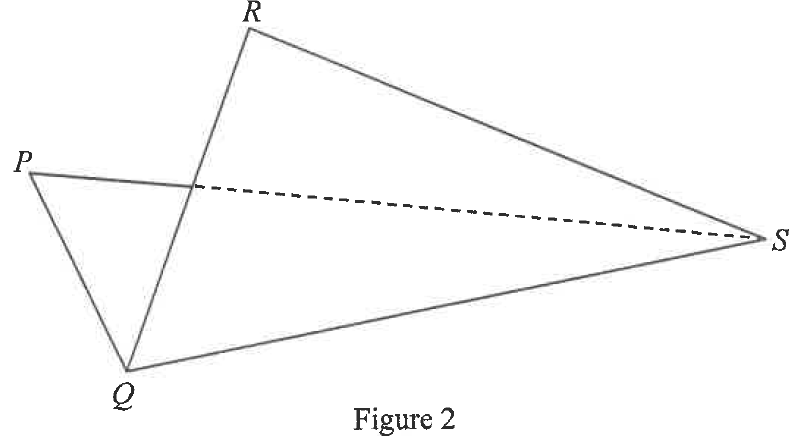
\includegraphics[width=0.5\linewidth]{figure_2.png}
                \end{figure}

                \begin{enumerate}[(i)]
                    \item 
                        Find the shortest distance from $R$ to the plane $PQS$.
                    \item
                        Let $X$ be any point lying on the plane $QRS$. Someone claims that the distance between $P$ and $X$ exceeds 8 cm. Is the claim correct? Explain your answer.
                \end{enumerate}
                \droppoints
        \end{parts}

    \label{2024-I-19: Graph transformation + ASGS}
    \question
        Let $\displaystyle f(x)= 2x^2 + 4mx + 8x + 2m^2 + 8m + n$, where $m$ and $n$ are real constants such that $mn < 0$. Denote the vertex of the graph of $y = f(x)$ by $P$.
        \begin{parts}
            \part[2]
                \vspace{0.2cm}
                Using the method of completing the square, express the coordinates of $P$ in terms of $m$ and $n$. \droppoints
            \part[2]
                \vspace{0.2cm}
                Describe the geometric meaning represented by transforming $f(x)$ to $\displaystyle f(\frac{x}{5}) + 7$. \droppoints
            \part[8]
                \vspace{0.2cm}
                Denote the vertex of the graph of $\displaystyle f(\frac{x}{5}) + 7$ by $Q$. Let $(a_1, b_1)$ and $(a_2, b_2)$ be the coordinates of $P$ and $Q$ respectively. Given that $a_1, 1+n, a_2$ is an arithmetic sequence, and $b_1, 4-m, b_2$ is a geometric sequence.
                \begin{enumerate}[(i)]
                    \item 
                        \vspace{0.2cm}
                        Find the coordinates of $P$ and $Q$.
                    \item
                        \vspace{0.2cm}
                        The coordinates of the points $R$ and $S$ are ($3t+27, t$) and ($3t+3, 2t-3$) respectively, where $t$ is a real number.

                        \vspace{0.2cm}
                        Is it possible that $PQRS$ is a rhombus? Explain your answer.
                \end{enumerate}
                \droppoints
        \end{parts}
\end{questions}
\end{document}